% The BLAKE3 chaining-value stack [BLAKE3, §5.1.2]: after k chunks the stack holds one complete
% subtree per 1-bit of k, newest (smallest) on top. Adding chunk k merges one subtree per
% trailing 1-bit of k. Shown for 1 to 6 chunks; each column is the stack after that many chunks.
% Original drawing for the Hash library.
\documentclass[tikz,border=6pt]{standalone}
\usepackage[T1]{fontenc}
\usepackage{lmodern}
% Shared style for the Hash diagrams.
% Palette: Okabe–Ito (colour-blind safe). Every diagram is drawn on an opaque white card so it
% stays legible on dark page themes.
\usetikzlibrary{arrows.meta,positioning,calc,fit,backgrounds}
\definecolor{hsblue}{HTML}{0072B2}
\definecolor{hsorange}{HTML}{E69F00}
\definecolor{hsgreen}{HTML}{009E73}
\definecolor{hsvermilion}{HTML}{D55E00}
\definecolor{hspurple}{HTML}{CC79A7}
\definecolor{hsink}{HTML}{1F2933}
\tikzset{
  >={Stealth[length=2.2mm]},
  every node/.style={font=\sffamily\small, text=hsink},
  wire/.style={draw=hsink, line width=0.6pt, ->},
  reg/.style={draw=hsink, line width=0.6pt, fill=hsblue!12, minimum width=9mm, minimum height=7mm},
  fn/.style={draw=hsink, line width=0.6pt, fill=hsorange!25, rounded corners=2pt, minimum width=10mm, minimum height=6mm},
  input/.style={draw=hsink, line width=0.6pt, fill=hsgreen!20, minimum width=9mm, minimum height=6mm},
  add/.style={circle, draw=hsink, line width=0.6pt, fill=white, inner sep=0pt, minimum size=5mm, font=\sffamily\bfseries},
  card/.style={fill=white, rounded corners=4pt},
}

\begin{document}
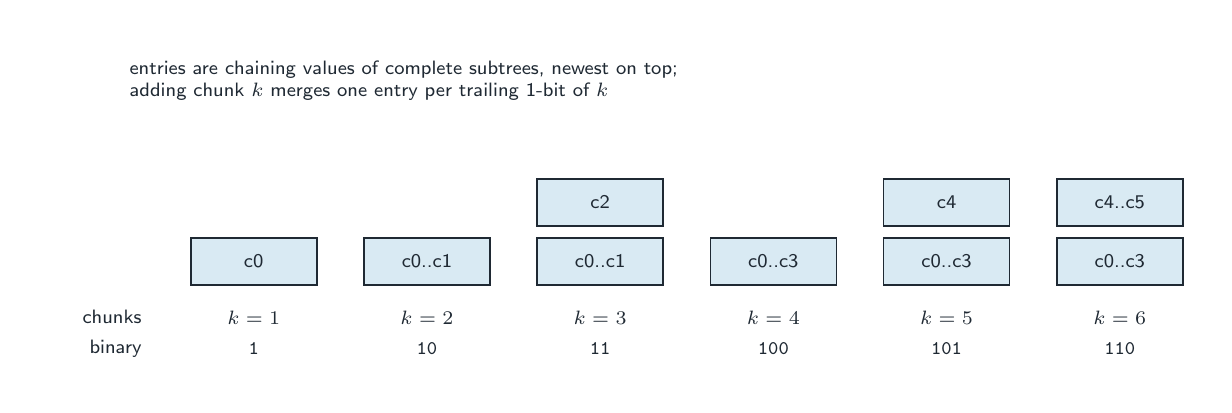
\begin{tikzpicture}[ent/.style={reg, minimum width=16mm, minimum height=6mm, font=\sffamily\scriptsize}]
  \def\dx{2.2}
  % Column k: entries bottom to top as "label/size".
  \foreach \k/\entries/\bin in {1/{c0}/1, 2/{c0..c1}/10, 3/{c0..c1,c2}/11, 4/{c0..c3}/100,
      5/{c0..c3,c4}/101, 6/{c0..c3,c4..c5}/110} {
    \foreach \e [count=\j from 0] in \entries {
      \node[ent, fill=hsblue!15] at (\k*\dx, \j*0.75) {\e};
    }
    \node[font=\sffamily\scriptsize, anchor=north] at (\k*\dx, -0.5) {$k = \k$};
    \node[font=\ttfamily\scriptsize, anchor=north] at (\k*\dx, -0.9) {\bin};
  }
  \node[font=\sffamily\scriptsize, anchor=east] at (0.9, -0.7) {chunks};
  \node[font=\sffamily\scriptsize, anchor=east] at (0.9, -1.1) {binary};
  \node[font=\sffamily\scriptsize, anchor=west, align=left] at (0.5, 2.3)
    {entries are chaining values of complete subtrees, newest on top;\\
     adding chunk $k$ merges one entry per trailing 1-bit of $k$};
  \begin{scope}[on background layer]
    \coordinate (e1) at (-0.6,-1.5);
    \coordinate (e2) at (6*\dx+1.0,2.9);
    \node[card, fit=(e1)(e2), inner sep=2pt] {};
  \end{scope}
\end{tikzpicture}
\end{document}
